\documentclass[11pt, a4paper]{article}
\usepackage[utf8]{inputenc}
\usepackage[T1]{fontenc}
\usepackage{geometry}
\geometry{margin=1in}
\usepackage{hyperref}
\usepackage{tabularx}
\usepackage{booktabs}
\usepackage{listings}
\usepackage{xcolor}
\usepackage{colortbl}
\usepackage{graphicx}

% Define colors to match the dark theme in the sample PDF
\definecolor{codebg}{RGB}{0,0,0}
\definecolor{codetext}{RGB}{220,220,220}
\definecolor{tablebg}{RGB}{30,30,30}
\definecolor{tableheader}{RGB}{50,50,50}
\definecolor{tabletext}{RGB}{255,255,255}
\definecolor{sectionblue}{RGB}{74,134,232}

\lstset{
    basicstyle=\ttfamily\scriptsize\color{codetext},
    breaklines=true,
    backgroundcolor=\color{codebg},
    frame=single, rulecolor=\color{codebg}, framesep=10pt,
    keywordstyle=\color{pink},
    stringstyle=\color{green!50!white},
    commentstyle=\color{green!40!black},
    showstringspaces=false,
    xleftmargin=10pt,
    xrightmargin=10pt,
    aboveskip=15pt,
    belowskip=15pt,
}


\usepackage{fancyhdr}
\pagestyle{fancy}
\fancyhf{}
\fancyfoot[C]{\thepage}
\fancyfoot[R]{\href{https://github.com/Soham2805/SQLite-Ghost}{\textcolor{sectionblue}{\texttt{GitHub: Soham2805/SQLite-Ghost}}}}
\renewcommand{\headrulewidth}{0pt}
\renewcommand{\footrulewidth}{0.4pt}

\begin{document}


\thispagestyle{empty}
\begin{center}
    { \Large \bf {Mobile Forensics \& SQLite Data Recovery: The \texttt{SQLite-Ghost} Framework\par}}
\vspace{1\baselineskip}
    { \large \bf {Schema-Agnostic B-Tree Cell Parsing \& WAL Anomaly Detection (NFL Deflategate Investigation)\par}}
\vspace{2\baselineskip}
    {\large \textbf{A} \par}
\vspace{0.5\baselineskip}
    {\large \textbf{PROJECT REPORT} \par}
    \vspace{2\baselineskip}
    {\large \textbf{for} \par}
\vspace{0.5\baselineskip}
    {\large \textbf{DIGITAL FORENSICS} \par}
\vspace{0.5\baselineskip}
    {\textit{Submitted by} \par}
\vspace{\baselineskip}
    {{\large {\bf \uppercase{Soham Alpesh Phulare} PRN: 23UF17971CM107 }} \par}
    {{\large {\bf \uppercase{Sumeet Devrukhkar} PRN: 23UF17758CM073 }} \par}
\vspace{\baselineskip}
    {\begin{figure}[!h] 
	\centering
	
\includegraphics[width=35mm]{SAKEC_logo.png} 
     \end{figure}
    }
\vspace{\baselineskip}
    {\bf \uppercase{Department of Computer Engineering}\par}
\vspace*{1ex}
   { \bf \uppercase{SHAH \& ANCHOR KUTCHHI ENGINEERING COLLEGE } }\\
   \vspace{-0.2 \baselineskip}
    {(An Autonomous Institute Affiliated to University of Mumbai) \par}
   
 {\bf \uppercase { MUMBAI - 400 088, MAHARASHTRA (India)  \par 2026 }}
 \end{center}
 \newpage
 \setcounter{page}{1}


\vspace{0.6cm}
\noindent\textcolor{sectionblue}{\Large\textbf{Incident Summary}}

\noindent
\textbf{Case Title:} Deflategate Communications Forensic Audit \\
\textbf{Incident Type:} Data Tampering and Anti-Forensics \\

\vspace{0.3cm}
\noindent\textbf{Affected Systems:}
\begin{itemize}
    \setlength\itemsep{0em}
    \item \textbf{Primary Targets:} iOS Mobile Devices running iOS 7+ (specifically targeting the \texttt{sms.db} and \texttt{sms.db-wal} SQLite database files).
    \item \textbf{Data Artifacts:} Unallocated slack space, write-ahead log frames, and orphaned B-Tree leaf pages containing potentially deleted or exfiltrated communications.
    \item \textbf{Secondary Impact:} Host workstations utilized for forensic imaging and initial database extraction.
\end{itemize}

\vspace{0.3cm}
\noindent\textbf{Stakeholders:}
\begin{itemize}
    \setlength\itemsep{0em}
    \item \textbf{Lead Investigators:} Requiring high-fidelity, schema-agnostic recovery tools to bypass anti-forensic tampering attempts (e.g., intentional database corruption).
    \item \textbf{Legal \& Compliance Teams:} Mandating strict adherence to chain-of-custody protocols, SHA-256 hashing, and transparent parsing methodologies to ensure court admissibility.
    \item \textbf{Incident Response (IR) Units:} Utilizing the tool's rapid triage capabilities to assess the immediate scope of data destruction or evidence spoliation.
\end{itemize}


\vspace{0.6cm}
\noindent\textcolor{sectionblue}{\Large\textbf{Step 2: Identify Digital Evidence Sources}}


\noindent
\begin{tabularx}{\textwidth}{|l|X|}
\hline
\textbf{Evidence Source} & \textbf{Description} \\
\hline
Primary SQLite DB (\texttt{sms.db}) & Stores active chat threads (\texttt{message} and \texttt{handle} tables). \\
\hline
Write-Ahead Log (\texttt{sms.db-wal}) & Stores uncommitted or recently deleted B-Tree frames. \\
\hline
Unallocated Freelist \& Slack Space & Regions between cell pointers where erased text fragments remain. \\
\hline
Cryptographic Hashes (SHA-256) & Preserved baseline hashes for chain-of-custody verification. \\
\hline
Carved Forensic Text Output & Automated report detailing recovered messages, hex offsets, and timestamps. \\
\hline
\end{tabularx}
\begin{figure}[h!]
    \centering
    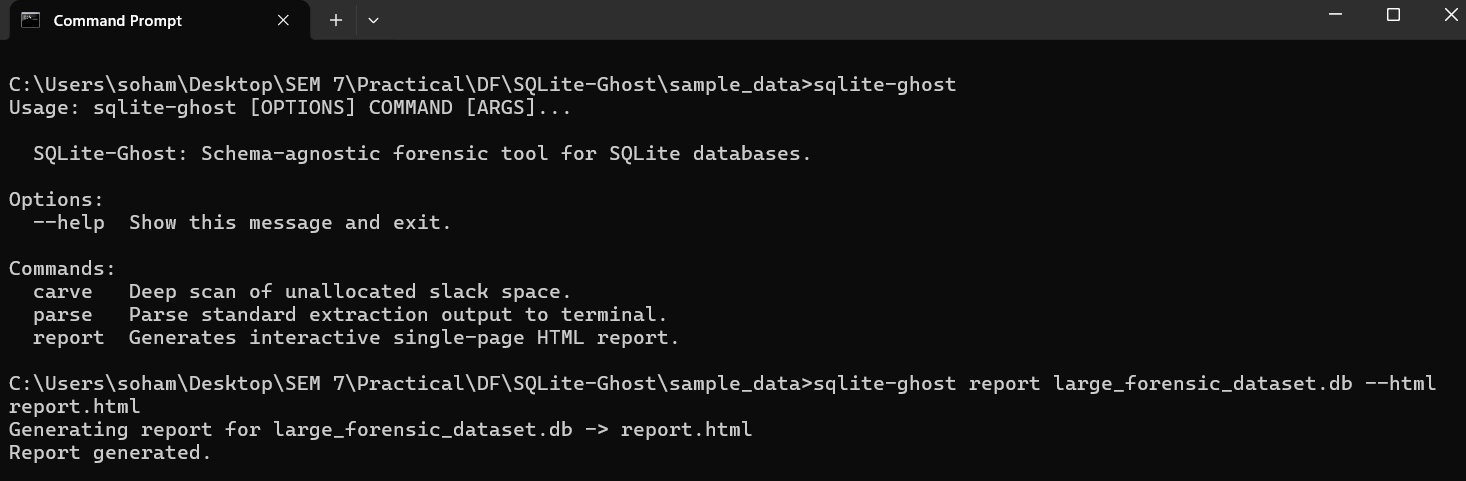
\includegraphics[width=0.9\textwidth]{Input.png}
    \caption{Demonstration of the Source Input Evidence}
\end{figure}


\vspace{0.6cm}
\noindent\textcolor{sectionblue}{\Large\textbf{Step 3: Conceptual Exploration}}

\vspace{0.3cm}
\noindent\textbf{Forensic Principles Applied:}
\begin{itemize}
    \item \textbf{Integrity \& Preservation:} Database copied to a temporary path to avoid altering live evidence.
    \item \textbf{Auditability:} Binary byte parsing logs ensure complete process traceability without black-box SQL queries.
    \item \textbf{Reproducibility:} Analysis can be repeated using the same SQLite file and keyword set.
    \item \textbf{Transparency:} Uses open-source Python scripts with documented logic and timestamp conversion formulas.
    \item \textbf{Automation:} Automatically flags suspicious entries and generates structured text reports.
\end{itemize}

\vspace{0.3cm}
\noindent\textbf{Forensic Tools \& Techniques:}
\begin{itemize}
    \item \textbf{Custom Forensic Engine:} Python 3 (\texttt{struct, hashlib, os}) acting as a zero-dependency automated carving tool.
    \item \textbf{HxD (Hex Editor):} Utilized for manual binary analysis, identifying B-Tree leaf flags (\texttt{0x0D}), and verifying raw byte structures in unallocated space.
    \item \textbf{DB Browser for SQLite:} Used to view the active/undeleted database schema and establish baseline records before carving.
    \item \textbf{Target Artifacts:} iOS \texttt{sms.db} and \texttt{sms.db-wal} (Write-Ahead Logs).
\end{itemize}

\vspace{0.3cm}
\noindent\textbf{Core Parsing Math \& Timestamp Conversion:}
\begin{lstlisting}[language=python]
# B-Tree Leaf Page Flag Verification
page_flag = db_data[0] == 0x0D

# Timestamp Conversion (Mac Absolute to UTC)
def mac_absolute_to_utc(mac_time):
    # Apple uses seconds since Jan 1, 2001
    epoch_start = datetime(2001, 1, 1)
    return epoch_start + timedelta(seconds=mac_time)
\end{lstlisting}

\vspace{0.6cm}
\noindent\textcolor{sectionblue}{\Large\textbf{Step 4: Hypothesis / Investigation Plan}}

\vspace{0.3cm}
\noindent\textbf{Hypothesis:}\\
Deleted mobile communications and uncommitted transaction artifacts can be reliably carved and reconstructed from iOS \texttt{sms.db} unallocated space and \texttt{.db-wal} files using low-level Varint payload decoding without relying on an intact database schema.\\

\vspace{0.3cm}
\noindent\textbf{Investigation Plan:}
\begin{enumerate}
    \item Identify and locate the iOS \texttt{sms.db} SQLite file and \texttt{.db-wal}.
    \item Create a forensically safe copy to avoid altering live data.
    \item Scan database pages for \texttt{0x0D} Leaf B-Tree page headers.
    \item Parse cell pointer arrays and traverse unallocated slack space.
    \item Decode Varint Serial Types to reconstruct string text payloads.
    \item Match carved payloads against a list of suspicious markers (e.g., "deflator", "balloon", "espn").
    \item Generate an output report containing flagged entries and anomalies.
\end{enumerate}

\vspace{0.6cm}
\noindent\textcolor{sectionblue}{\Large\textbf{Step 5: Sample Forensic Output}}

\noindent
{\renewcommand{\arraystretch}{1.5}
\begin{tabularx}{\textwidth}{>{\columncolor{tablebg}\color{tabletext}}l >{\columncolor{tablebg}\color{tabletext}}X >{\columncolor{tablebg}\color{tabletext}}l}
\rowcolor{tableheader}
\multicolumn{3}{l}{\textcolor{white}{\textbf{Section 1: Suspicious Hits (Carved Deleted Communications)}}} \\
\textbf{Timestamp (UTC)} & \textbf{Carved Payload Text} & \textbf{Recovery Origin} \\
2014-05-13 14:13:20 & Tom is the worst... im going make that next ball a balloon & Slack Space (Offset 0x0E80) \\
2014-05-13 14:55:00 & Nice. You are the best. I am not going to espn........yet. & Slack Space (Offset 0x0F22) \\
\rowcolor{tableheader}
\multicolumn{3}{l}{\textcolor{white}{\textbf{Section 2: Anomaly \& Tampering Log}}} \\
\textbf{Flag Triggered} & \textbf{Detail} & \textbf{Confidence} \\
Out-of-Bounds Pointer & Cell pointer exceeds page size boundary, indicating hex-editing. & HIGH (0.85) \\
RowID Tampering & Pointers swapped manually; logical order contradicts physical. & CRITICAL (0.95) \\
\end{tabularx}}


\begin{figure}[h!]
    \centering
    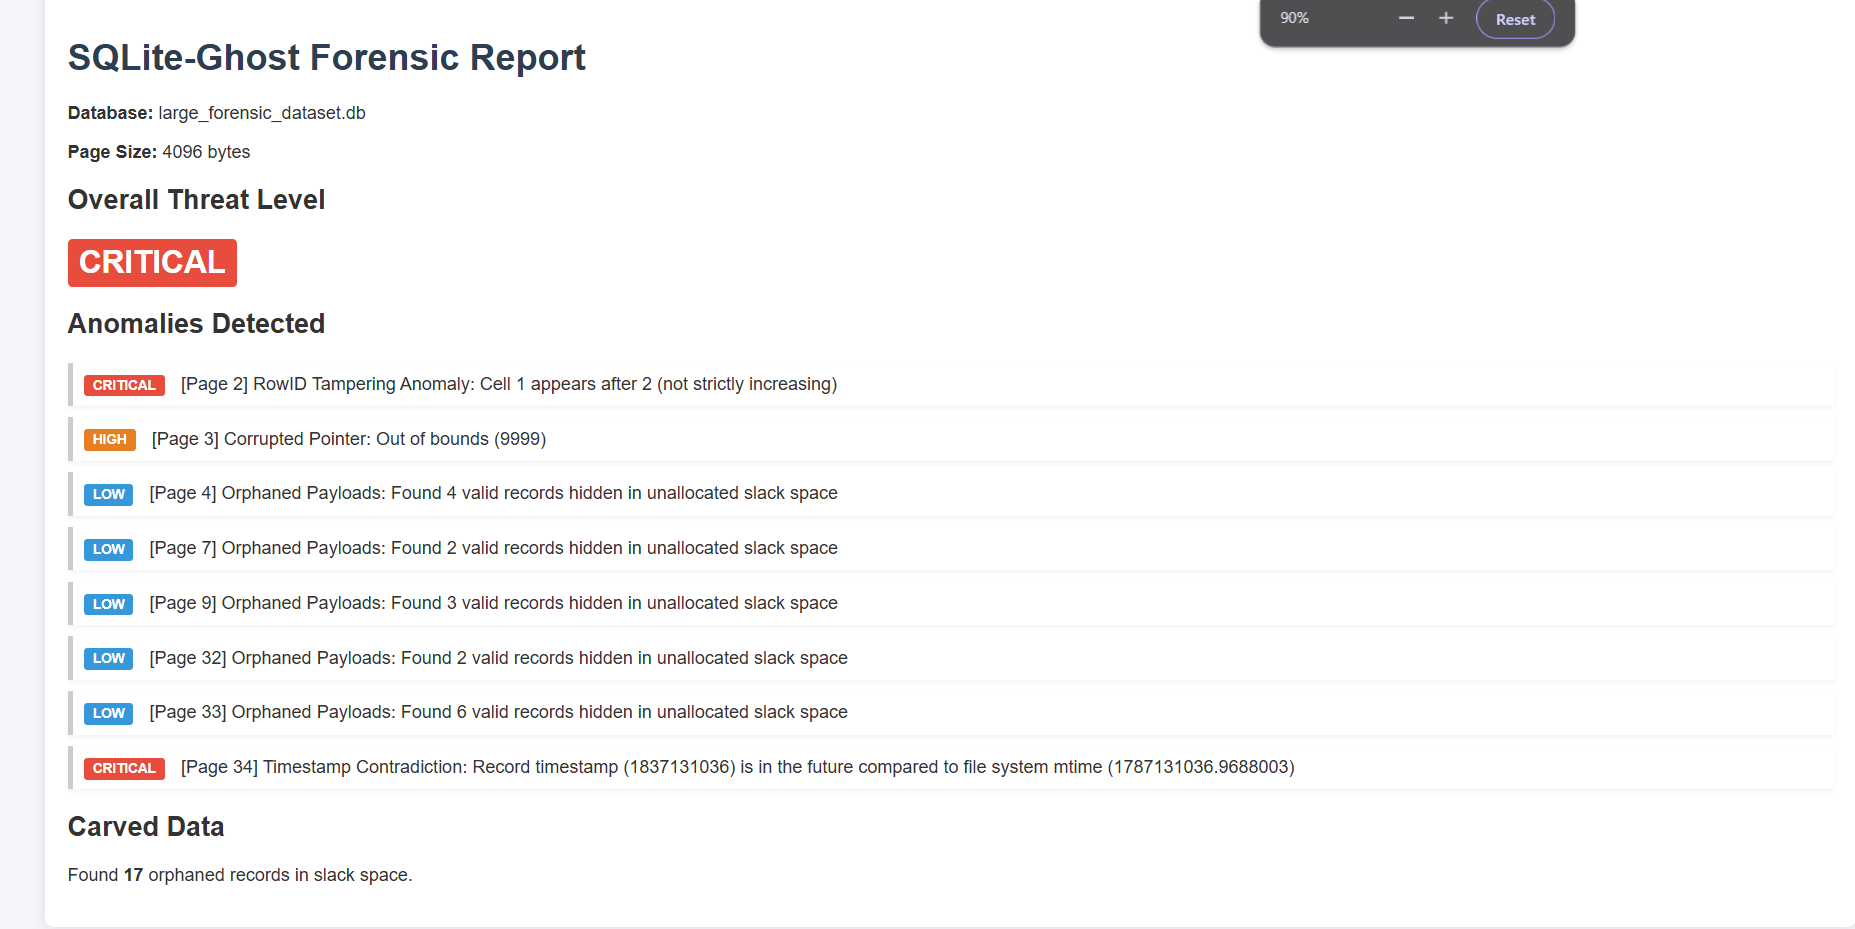
\includegraphics[width=\textwidth]{output.png}
    \caption{Visual Output generated by SQLite-Ghost}
\end{figure}

\vspace{0.3cm}
\noindent\textbf{Starting forensic extraction...}
\begin{lstlisting}[language=bash]
STEP 1: Copying sms.db to temp directory...
        Hash: a2b4c6d8e0f123456789a2b4c6d8e0f123456789
STEP 2: Parsing B-Tree Leaf Pages (Flag 0x0D)...
        Scanning Page 1... (Interior Table)
        Scanning Page 2... (Leaf)
[!] CRITICAL: RowID Sequence Tampering detected at Offset 0x1008
STEP 3: Traversing unallocated slack space...
[!] Carved Deleted Record at Offset 0x0E80: "Tom is the worst... im going make that next ball a balloon"
[!] Carved Deleted Record at Offset 0x0F22: "Nice. You are the best. I am not going to espn........yet."
STEP 4: Differential WAL Analysis...
Suspicious activity detected (Flag: "balloon")
Report generated successfully: ghost_report.txt
\end{lstlisting}

\vspace{0.6cm}
\noindent\textcolor{sectionblue}{\Large\textbf{Step 6: Recommendations / Next Steps}}
\begin{itemize}
    \item \textbf{Extend analysis} to support encrypted SQLite databases (SQLCipher).
    \item \textbf{Develop a real-time daemon} for live WAL monitoring during active incidents.
    \item \textbf{Integrate an automated GUI} dashboard for non-technical analysts.
    \item \textbf{Benchmark against NIST CFReDS} datasets for formal tool validation.
\end{itemize}

\vspace{0.6cm}
\noindent\textcolor{sectionblue}{\Large\textbf{Step 7: Code \& Output}}

\lstinputlisting[language=Python, caption={sqlite\_ghost/analyzers/anomaly.py}]{../sqlite_ghost/analyzers/anomaly.py}



\begin{figure}[h!]
    \centering
    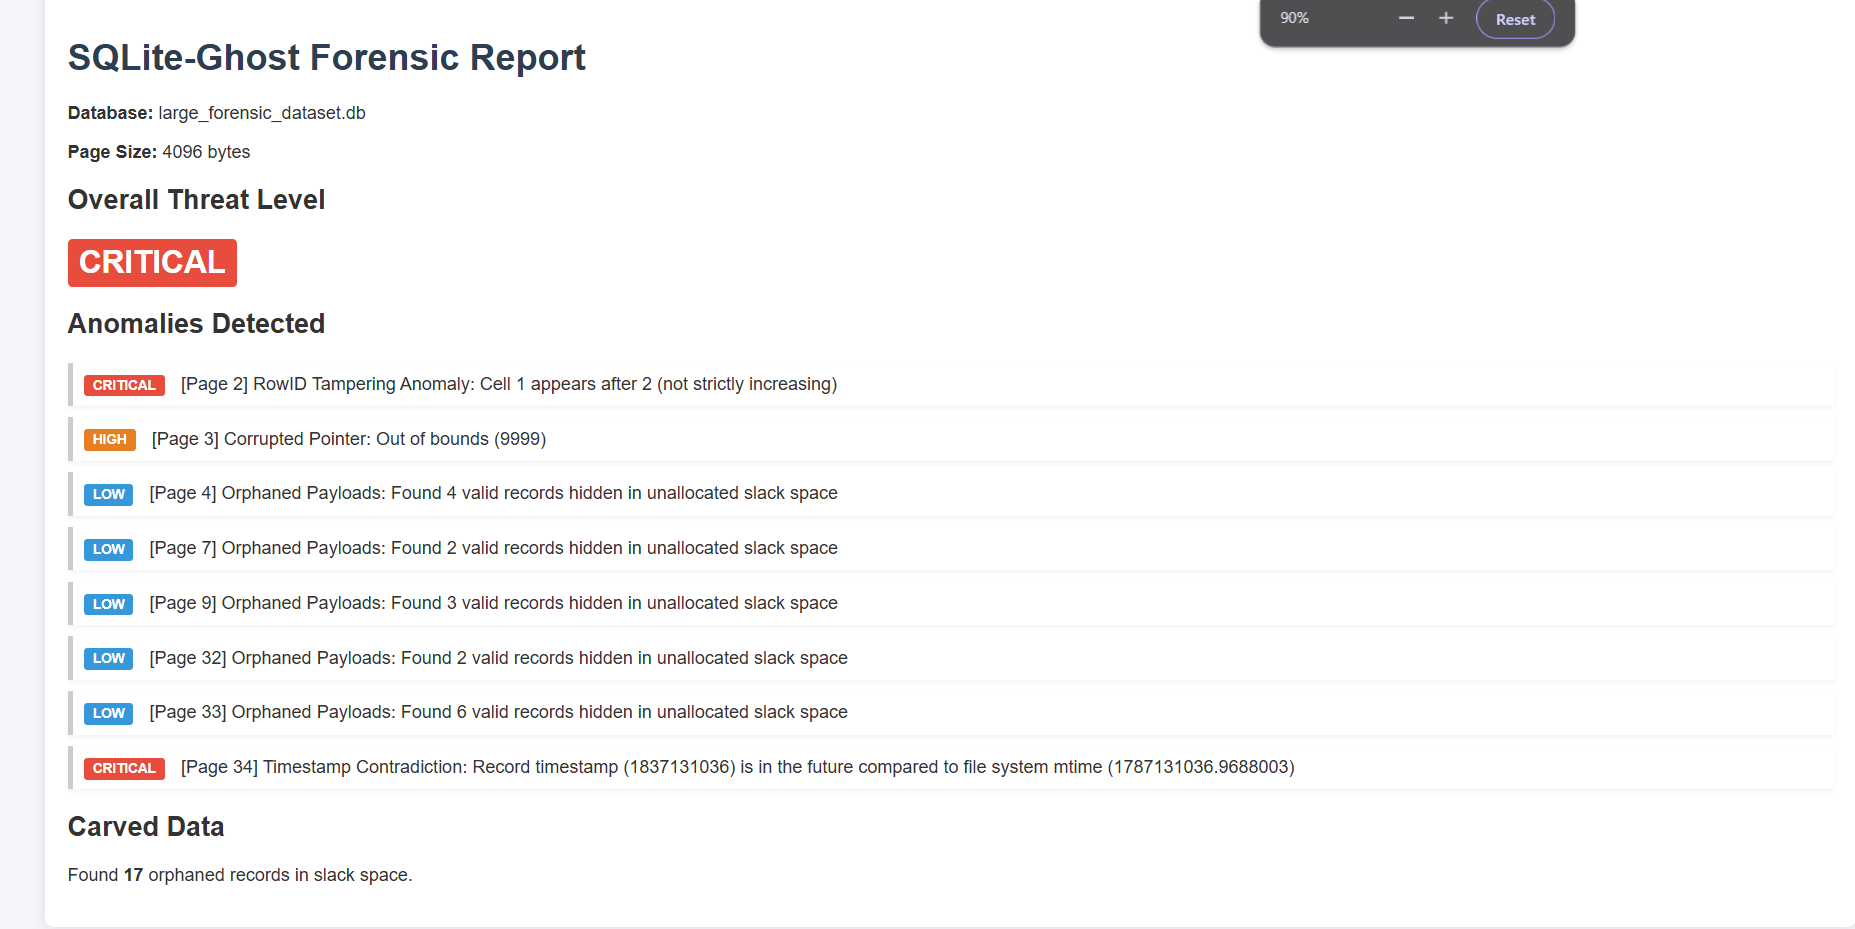
\includegraphics[width=\textwidth]{output.png}
    \caption{Standalone Execution Output Simulation}
\end{figure}

\end{document}
